%!TEX root = ../nwoods_thesis.tex

\chapter{The CMS Experiment and the CERN LHC}
Production of controlled high-energy particle collisions, and detection of the decay products resulting from those collisions, are monumental technical challenges. The apparatus used to obtain the results presented in this thesis are the result of decades of work by thousands of scientists and engineers, making use of many techniques developed in the course of building and operating previous experiments. The CERN Large Hadron Collider (LHC)~\cite{Evans:2008zzb,Bruning2012705} accelerates pairs of charged hadron (proton or lead ion) beams to high energies and collides them to provide a source of data to several fully independent detectors, including the Compact Muon Solenoid (CMS)~\cite{Chatrchyan:2008zzk}, which collected the data used in the studies presented here. Detailed descriptions of the LHC and CMS follow.


%-------------------------------------------------------------------------------
% LHC
%-------------------------------------------------------------------------------

\section{The CERN Large Hadron Collider}
The LHC, the most powerful particle accelerator and collider ever built, is a $26.7\unit{km}$ circumference ring of superconducting magnets running through tunnels roughly $100\unit{m}$ below the suburbs and countryside near Geneva, Switzerland.
It first produced collisions suitable for collecting physics data in 2010 before generating large datasets with beam energies of $3.5\TeV$ in 2011 and $4\TeV$ in 2012.
Following a shutdown for upgrades an repairs, it returned in 2015 and 2016 to deliver beam energies of $6.5\TeV$.
Beams collide head-on so that the center-of-mass frame of the proton-proton system is the rest frame of the detectors, giving proton-proton center-of-mass energies of 7, 8, and $13\TeV$ respectively for collisions in 2010--2011, 2012, and 2015--2016.
Each successive energy was the highest ever acheived in controlled proton-proton collisions, giving unprecedented access to extremely high-energy processes at every step.

In addition to increasing collision energies, the LHC increased its rate of collisions with each new machine configuration.
The average event rate $\ddinline{N}{t}$ for a process with production cross section $\sigma$ is determined by the instantaneous luminosity $\lumiL$ of the collider,
\begin{equation}
  \label{eq:instLumi}
  \dd{N}{t} = \lumiL\sigma
\end{equation}
so a high instantaneous luminosity is vital to the timely observation of rare processes like Higgs boson production.
The LHC's unprecedented luminosities have allowed collection of the largest physics datasets in history.

The desire for high luminosities drove the decision to collide protons with other protons instead of with antiprotons as was done at Tevatron, LHC's predecessor at Fermilab in Batavia, IL\@.
Antiprotons simply cannot be produced in sufficient quantities for a collider on this scale.
Many of the physics processes Tevatron was designed to study are $\Pq\Paq$-initiated, so it is useful to have valence antiquarks available in the collisions.
The LHC was designed with Higgs boson production in mind, and the two most important Higgs production modes are proton/antiproton agnostic.
Even for $\Pq\Paq$-initiated processes, valence antiquarks are less critical at the LHC because, for equal parton momenta, protons have larger antiquark content at LHC energies than at Tevatron energies ($1.98\TeV$ center-of-mass energy) as discussed in Section~\ref{sec:pp}.

In addition to protons, the LHC can accelerate beams of lead nuclei to $2.51\TeV$ per nucleon, also the highest ever achieved.
All studies presented in this thesis were performed on proton-proton collision data, rendering the details of so-called ``heavy ion'' beams beyond the scope of this document.

Beams are maintained and manipulated with magnets, most of them made of superconducting niobium-titanium (NbTi) winding cooled to $1.9\unit{K}$ by superfluid helium.
Dipole magnets with fields up to $8.33\unit{T}$ bend the beam around the ring, interspersed with quadrupoles for focusing.
More quadrupoles and higher-moment magnets keep the beams focused, squeeze them for collisions, and apply a number of corrections.
Superconducting radio frequency (RF) cavities operating at $400\unit{MHz}$ accelerate the beam, maintain it at its final energy, and maintain bunch shape and spacing.


\subsection{Accelerator Chain, Layout, and Detectors}
The LHC was built in tunnels originally constructed for the Large Electron-Positron Collider (LEP), an $\Pe^+$-$\Pe^-$ collider that operated from 1989 to 2000.
Using existing caverns, tunnels, and infrastructure was a substantial cost-saving measure, but imposed several important constraints on the LHC's design.
In LEP, the electron and positron beams could be accelerated in opposite directions by the same magnets, because they are oppositely charged.
Conversely, proton beams require opposite magnetic fields for the two beams.
Because the tunnels were not wide enough to accommodate two completely separate beam lines, most of the magnets in the LHC use a twin-bore design, shown schematically in Fig.~\ref{fig:lhcDipole}, in which the pipes and windings for the two beams share a common cryogenic system.
The electromagnetic, mechanical, and cryogenic coupling of the two beamlines represents a significant engineering challenge.

\begin{figure}[h]
  \centering
  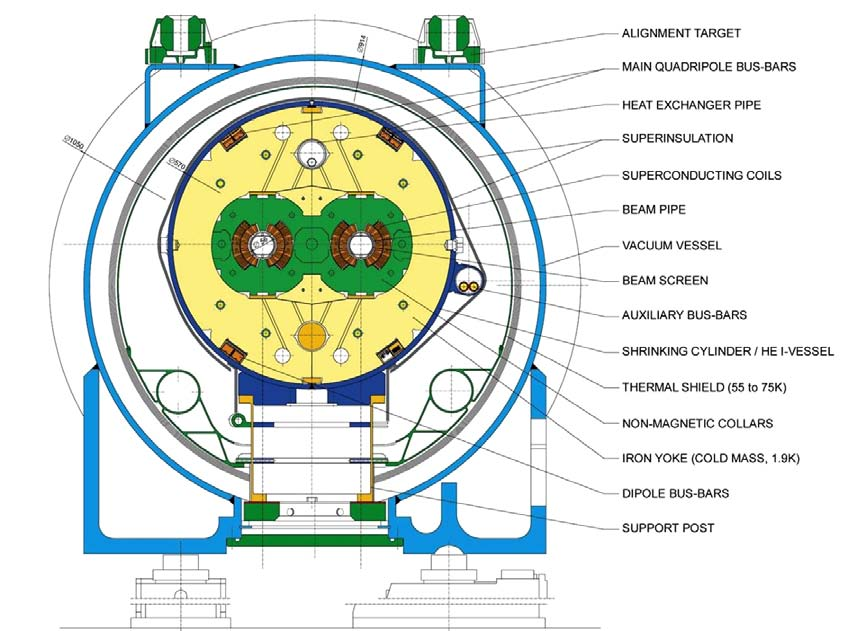
\includegraphics[width=0.8\textwidth]{experiment/lhcDipole.png}
  \caption{
    Schematic cross section of an LHC dipole and its attendent electrical and cryogenic infrastructure, reproduced from Ref.~\cite{Evans:2008zzb}.
    }\label{fig:lhcDipole}
\end{figure}

Because no single accelerator has the dynamic range necessary to take a stationary proton to \TeV-scale energies, a chain of smaller accelerators repurposed from previous experiments feeds moderate-energy protons into LHC\@.
Protons are obtained by ionizing hydrogen atoms, then accelerated to $50\MeV$ by the Linac~2 linear accelerator and injected into the Proton Syncrotron Booster~(PSB), the first of several circular accelerators.
The PSB feeds $1.4\GeV$ protons into the Proton Synchrotron~(PS), which in turn injects them into the Super Proton Synchrotron~(SPS) at $26\GeV$.
The protons are then accelerated to $450\GeV$ in the SPS before being injected into LHC\@.
A diagram of the entire accelerator chain is shown in Fig.~\ref{fig:acceleratorChain}.

\begin{figure}[h]
  \centering
  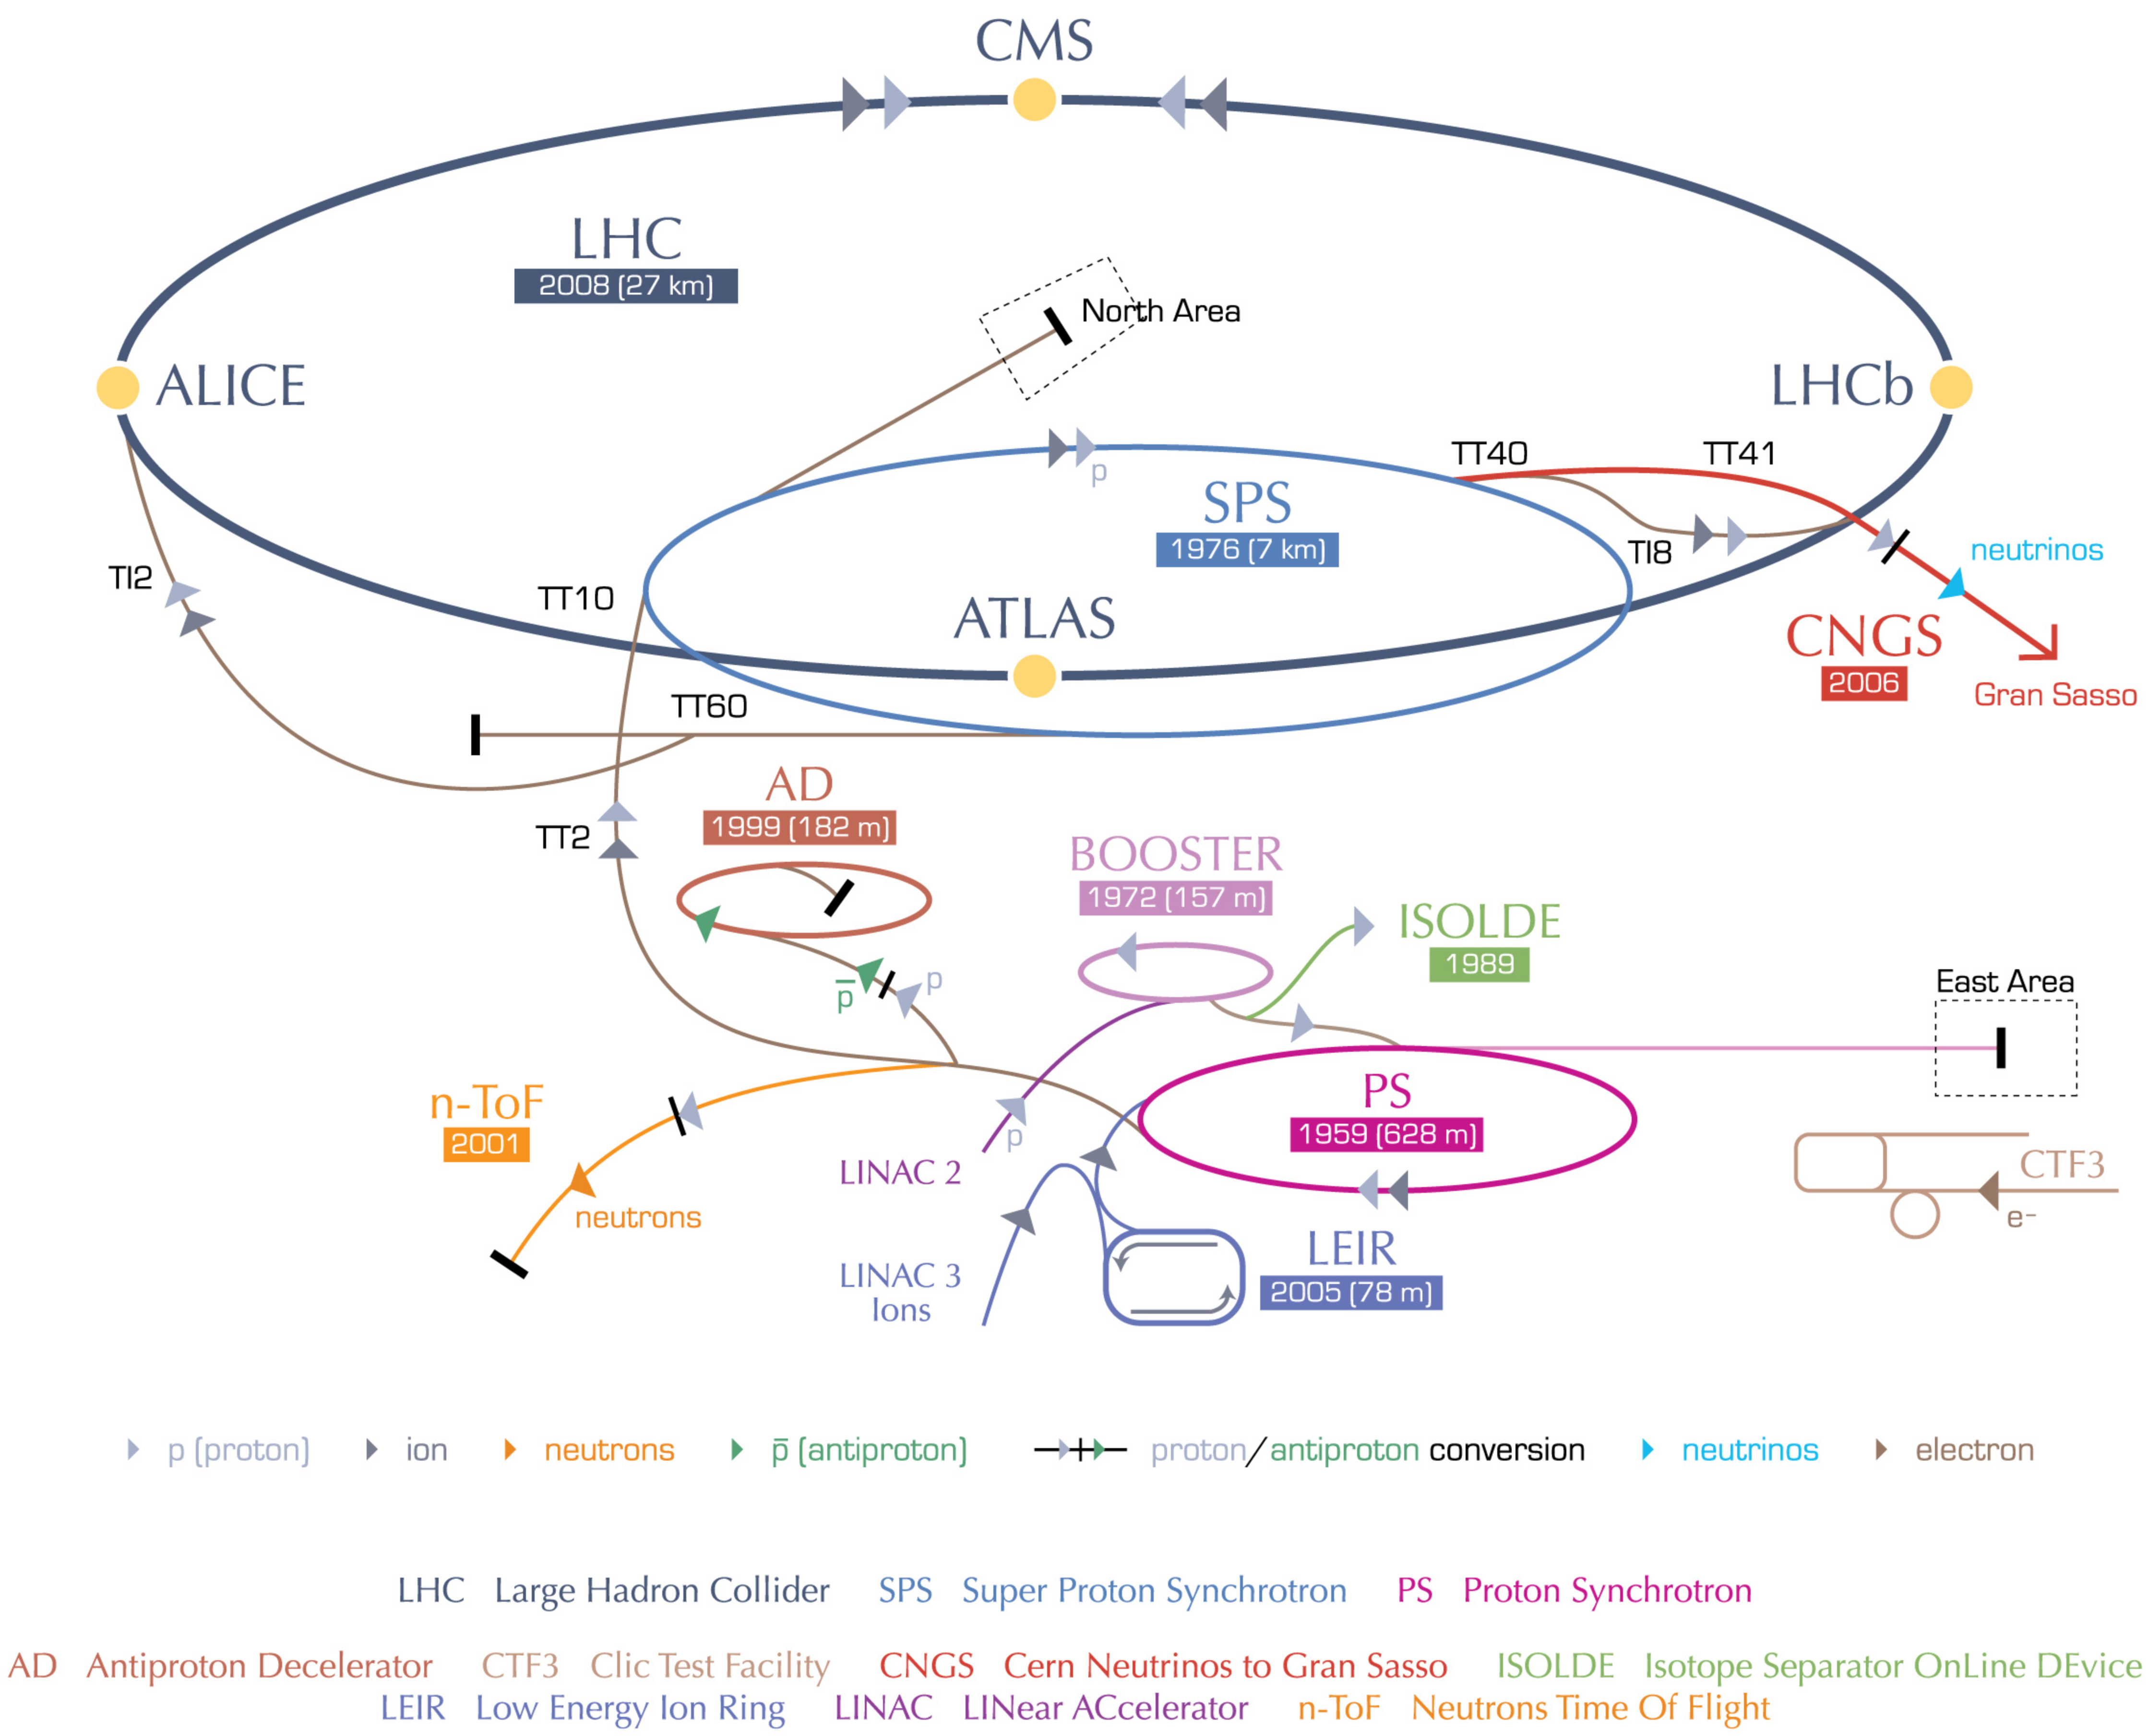
\includegraphics[width=\textwidth]{experiment/acceleratorChain.png}
  \caption{
    A schematic of the LHC accelerator chain and peripheral experiments, reproduced from Ref.~\cite{Christiane:1260465}.
  }\label{fig:acceleratorChain}
\end{figure}

The ring is divided into eight sectors, each of which features a $528\unit{m}$ straight section connected to the adjacent sections by $2.45\unit{km}$ arcs.
The straight section length was set by the need for RF cavities to accelerate LEP beams to counteract synchrotron radiation, which is a primary factor limiting electron and positron beam energy.
This is not ideal for proton beams; protons' much higher mass means they radiate less and need fewer RF cavities.
The straight sections feature ``insertion'' points numbered with Point~1 at the main CERN site in Meyrin, Switzerland, and the rest numbered~2--8, increasing in the clockwise direction when viewed from above.
Points~1, 2, 5, and~8 have beam crossing points and host detectors to study the resulting proton-proton collisions.
Points~3 and~7 feature collimators to remove nonuniformities in the beams.
The RF cavities are at Point~4 and the beams are dumped after use into absorbers at Point 6\@.

The CMS detector is at Point~5 in Cessy, France, the furthest point on the ring from the Meyrin site and Point~1, which houses ATLAS~\cite{Aad:2008zzm}, a similar but fully independent general-purpose particle detector.
CERN and the science funding agencies support CMS and ATLAS equally so that any measurement or discovery made by one can be made concurrently or verified by the other.
The other two experimental insertions feature specialized detectors studying collisions at lower-luminosity beam interaction points.
The LHCb detector~\cite{Alves:2008zz}, at Point~8, studies hadronic physics with an emphasis on b-mesons, and ALICE~\cite{Aamodt:2008zz} studies heavy ion collisions at Point~2\@.
Three smaller experiments share interaction points with the larger detectors, with TOTEM~\cite{Anelli:2008zza} studying proton structure and the total proton-proton interaction cross section next to CMS\@; LHCf~\cite{Adriani:2008zz} studying the $\pi^0$ energy spectrum and multiplicity near ATLAS\@; and MoEDAL~\cite{Acharya:2014nyr} searching for magnetic monopoles or other heavy, stable, ionizing particles at Point~8 with LHCb.



\subsection{Operating Parameters}
With the beam energy set by the radius of the ring and the strength of available magnets, the number of interesting physics events produced in LHC collisions depends only on the integrated luminosity
\begin{equation}
  \lumiL_\textit{int} = \int \lumiL \cmsSymbolFace{d}t,
\end{equation}
where $\lumiL$ is the instantaneous luminosity defined in Eq.~\ref{eq:instLumi} and the integral runs over the time the machine spends in collisions mode.
LHC's availability for collisions depends on the electrical and mechanical stability of the accelerators and their support systems, including the cryogenics and the vacuum in the beam pipe.
The instantaneous luminosity while running depends only on the beam parameters.
For symmetric beams which each have $n_b$ colliding gaussian bunches of intensity (i.e.\ number of protons in the bunch) $N_b$, orbiting the ring with frequency $f_\textit{rev}$ and relativistic factor $\gamma=E_p/m_p$, the instantaneous luminosity is give by
\begin{equation}
  \lumiL = f_\textit{rev} \frac{n_b N_b^2 \gamma}{4\pi \beta^\ast \epsilon_N} R,
\end{equation}
where $\beta^\ast$ is the amplitude of the beams' betatron oscillations around the nominal ring path at the interaction point, the normalized emittance $\epsilon_N$ is a measure of the beams' spread in both position and momentum space, and $R$ is a geometrical factor accounting for the beam crossing angle,
\begin{equation}
  R = \sqrt{1 + \left(\frac{\theta_c \sigma_z}{2\sigma^\ast}\right)^2}.
\end{equation}
Here $\theta_c$ is the beams' crossing angle, and $\sigma_z$ and $\sigma^\ast$ are respetively the longitudinal and transverse RMS widths of the bunches in the lab frame.


\subsubsection{Design}
The machine parameters in the LHC design specification can be seen in the first column of Table~\ref{tab:lhcparams}.
Many of the design parameters, in particular the energy and number of colliding bunches, have not been met due to a failure during initial testing in September 2008.
A fault in a superconducting bus bar connection between a dipole and a quadrupole caused an electrical arc which ruptured the cryostat, leading to a rapid and destructive release of helium gas~\cite{Bajko:1168025}.
When LHC was brought back online in 2010 after repairs and upgrades intended to prevent similar incidents in the future, its operating parameters were changed to further reduce the risk of catastrophic failure.
Some luminosity-related parameters were adjusted to mitigate the resulting loss of physics discovery potential as much as possible.
Further upgrades have improved machine performance, with some parameters now meeting or exceeding the design specification.


\begin{table}
\caption{
  LHC beam parameters as designed and in practice.
  As stated in the text, $n_b$ is the number of colliding bunches, $N_b$ is the number of protons in each bunch, $\beta^\ast$ is the betatron amplitude at the interaction point, $\epsilon_N$ is the normalized emittance, and $\lumiL_{\left(\textit{int}\right)}$ is the instantaneous (integrated) luminosity.
  }
\centering
\begin{tabular}{lllllll}
\toprule
                                                                     & \multicolumn{1}{c}{Design} & \multicolumn{3}{c}{Run I}  & \multicolumn{2}{c}{Run II} \\
\midrule
Year                                                                 &          & 2010    & 2011    & 2012    & 2015    & 2016                               \\
\midrule\midrule
Energy per beam $\left(\TeVns\right)$                                & 7        & 3.5     & 3.5     & 4       & 6.5     & 6.5                                \\
Bunch spacing $\left(\unitns{ns}\right)$                             & 25       & 150     & 50      & 50      & 25      & 25                                 \\
$n_b$                                                                & 2808     & 348     & 1331    & 1368    & 2232    & 2208                               \\
$N_b \left(10^{11}\right)$                                           & 1.15     & 1.2     & 1.5     & 1.7     & 1.15    & 1.25                               \\
$\beta^\ast \left(\unitns{m}\right)$                                 & 0.55     & 3.5     & 1.0     & 0.6     & 0.8     & 0.4                                \\
$\epsilon_N \left(\unitns{mm}\unit{mrad}\right)$                     & 3.75     & 2.2     & 2.3     & 2.5     & 3.5     & 3.0                                \\
Peak pileup                                                          & FIXME    & 4       & 17      & 37      & 22      & 49                                 \\
Peak $\lumiL \left(10^{34}\unitns{cm}^{-2}\unitns{s}^{-1}\right)$    & 1        & 0.02    & 0.35    & 0.77    & 0.52    & 1.53                               \\
$\lumiL_\textit{int} \left(\fbinvns\right)$                          &          & 0.04    & 6.1     & 23.3    & 4.2     & 41.1                               \\
\bottomrule

\end{tabular}\label{tab:lhcparams}
\end{table}


\subsubsection{Run I}
The LHC was brought back online in 2010 at half its design energy, with $3.5\TeV$ beam energy, which was increased to $4\TeV$ in 2012. The bunch intensity was also lower, with bunches spaced $50\unit{ns}$ apart instead of $25\unit{ns}$.
The longer bunch spacing was chosen to allow full exploitation of excellent injection chain performance~\cite{1742-6596-455-1-012001}.
Beams exiting the SPS had bunch intensity as much as 50\% higher than anticipated in the original LHC design and beam emittance as low as 67\% of nominal.
This allowed the LHC to achieve 77\% of its design instantaneous luminosity in 2012 despite having roughly half as many bunches in each beam.

Machine availability was overall good considering the complexity and relative newness of the LHC, with about 36\% of scheduled time spent in stable beams.
In all, LHC delivered $6.1\fbinv$ to CMS and ATLAS in 2011 and $23.3\fbinv$ in 2012, enough to allow discovery of the Higgs boson.
The integrated luminosity for each year of LHC operation is shown as a function of calendar month and day in Fig.~\ref{fig:intLumi}.

\begin{figure}[h]
  \centering
  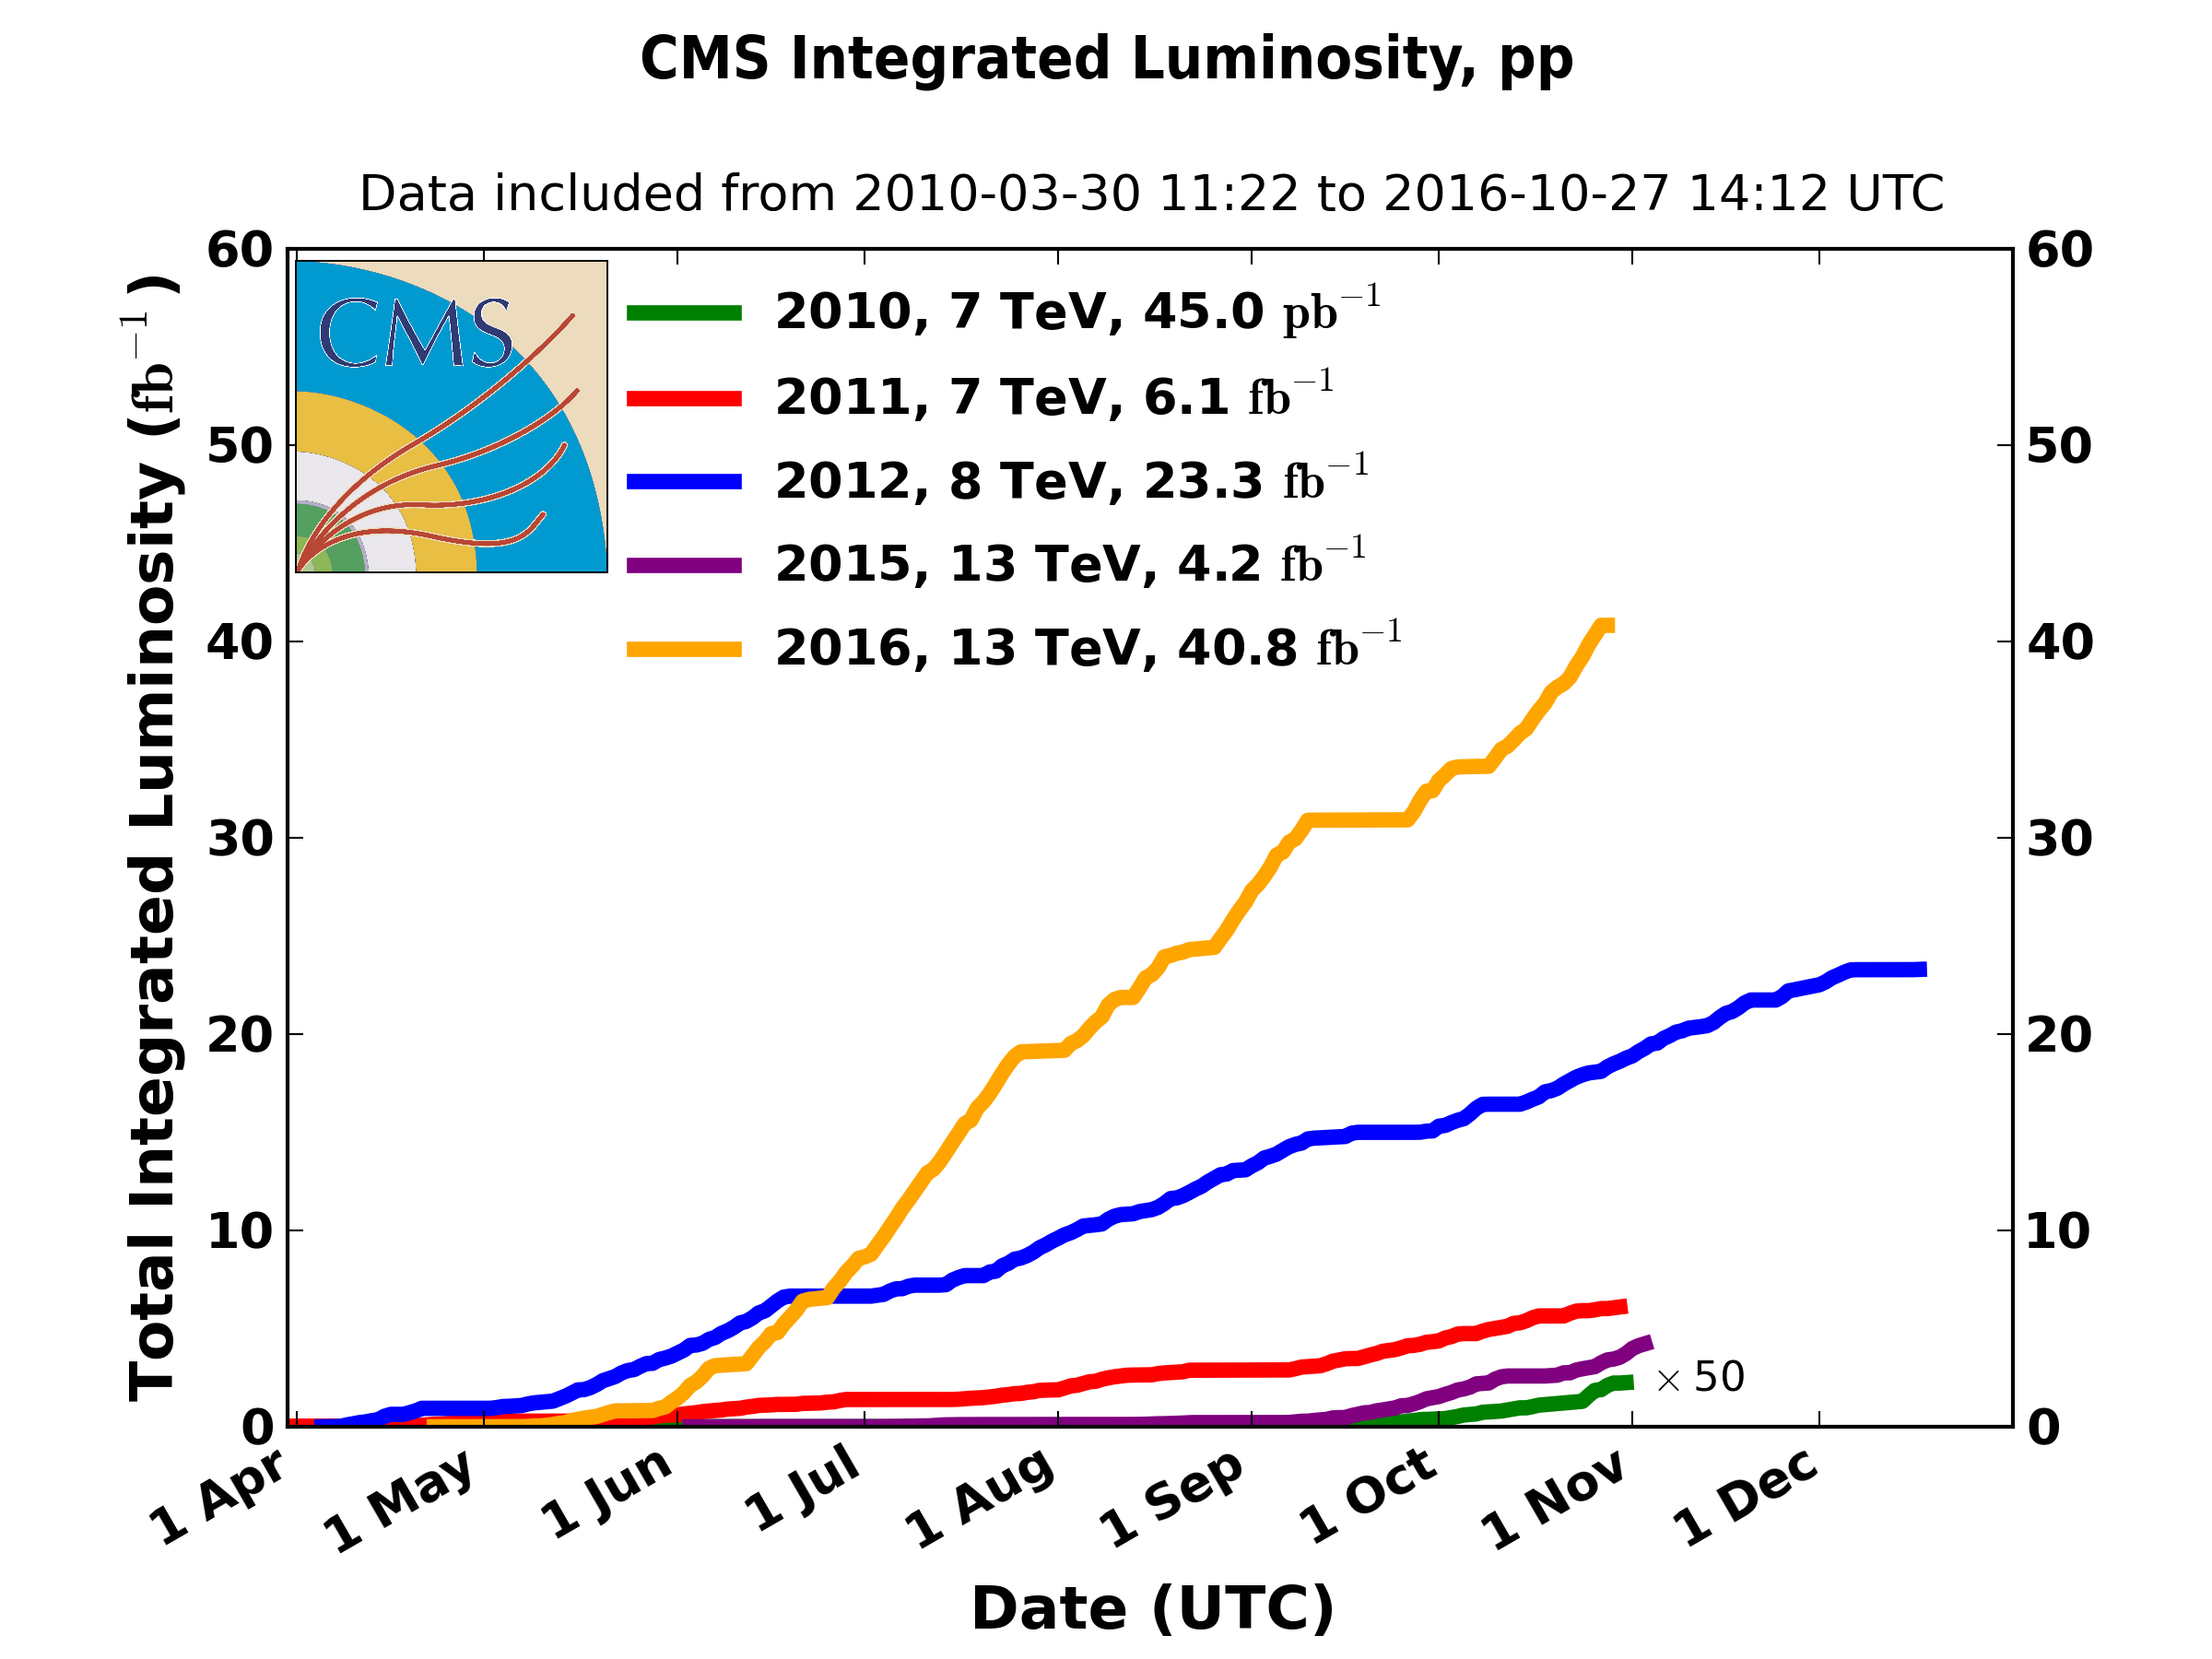
\includegraphics[width=.7\textwidth]{experiment/intLumi.png}
  \caption{
    The integrated luminosity delivered to CMS in each year of LHC operation, shown as a function of the date within the year.
  }\label{fig:intLumi}
\end{figure}


\subsubsection{Run II}
The LHC shut down for 2013 and 2014 to allow a number of repairs and upgrades, including measurements, repairs and upgrades on the electrical connections and cryogenic safety systems like the ones that failed in 2008\@.
Beam energies could then be increased to $6.5\TeV$, close to the nominal $7\TeV$.
The bunch spacing was decreased to $25\unit{ns}$ while maintaining low emittance and high bunch intensity with the implementation of the beam compression merging and splitting (BCMS) scheme in which bunches are merged in the PS before they are split for injection into SPS, allowing higher bunch intensity~\cite{Papaphilippou:2014qwa}.
This was offset by vacuum problems in the SPS beam dump, which limited the total number of colliding bunches to around 2200~\cite{Frederick:2235979}.
Improvements in collimators and beam optics reduced $\beta^\ast$ to $40\unit{cm}$ in 2016, lower than the design $\beta^\ast$ of $55\unit{cm}$.
Overall instantaneous luminosities were substantially higher than originally designed.

Machine availability in Run II was excellent, with over 60\% of planned time spent in stable beams~\cite{Frederick:2235979}.
Mechanical problems kept LHC out of commission for much of 2015, and only $4.2\fbinv$ were delivered to Points~1 and~5, but the integrated luminosity in 2016, $41.1\fbinv$, was far above the roughly $25\fbinv$ expected and more than all previous runs combined.



%-------------------------------------------------------------------------------
% CMS
%-------------------------------------------------------------------------------

\section{The Compact Muon Solenoid Detector}
The CMS detector~\cite{Chatrchyan:2008zzk} is a general-purpose particle detector located in a cavern roughly $100\unit{m}$ below LHC Point~5.
Though designed to do a wide range of physics analyses, CMS was designed specifically with Higgs boson discovery in mind.
Primary design goals include
\begin{itemize}
  \item High-efficiency reconstruction of charged particles with precise measurement of their trajectories and momenta
  \item Good electromagnetic energy resolution, including diphoton and dielectron mass resolution
  \item Hermetic calorimetry for good missing transverse energy and dijet mass resolution
  \item Good muon identification, momentum resolution (including dimuon mass resolution), and charge determination over a broad range of energies
\end{itemize}
To this end, CMS features a silicon tracker, a scintillating crystal electromagnetic calorimeter (ECAL), and a hermetic hadronic calorimeter (HCAL) inside a $3.8\unit{T}$ solenoid magnet surrounded by ionized gas muon tracking devices, all of which can be seen as part of the whole detector in Fig.~\ref{fig:cmsWhole}.
Decisions on which events to read out are made on-line by a two-level trigger system.
Descriptions of these systems follow.

\begin{figure}[h]
  \centering
  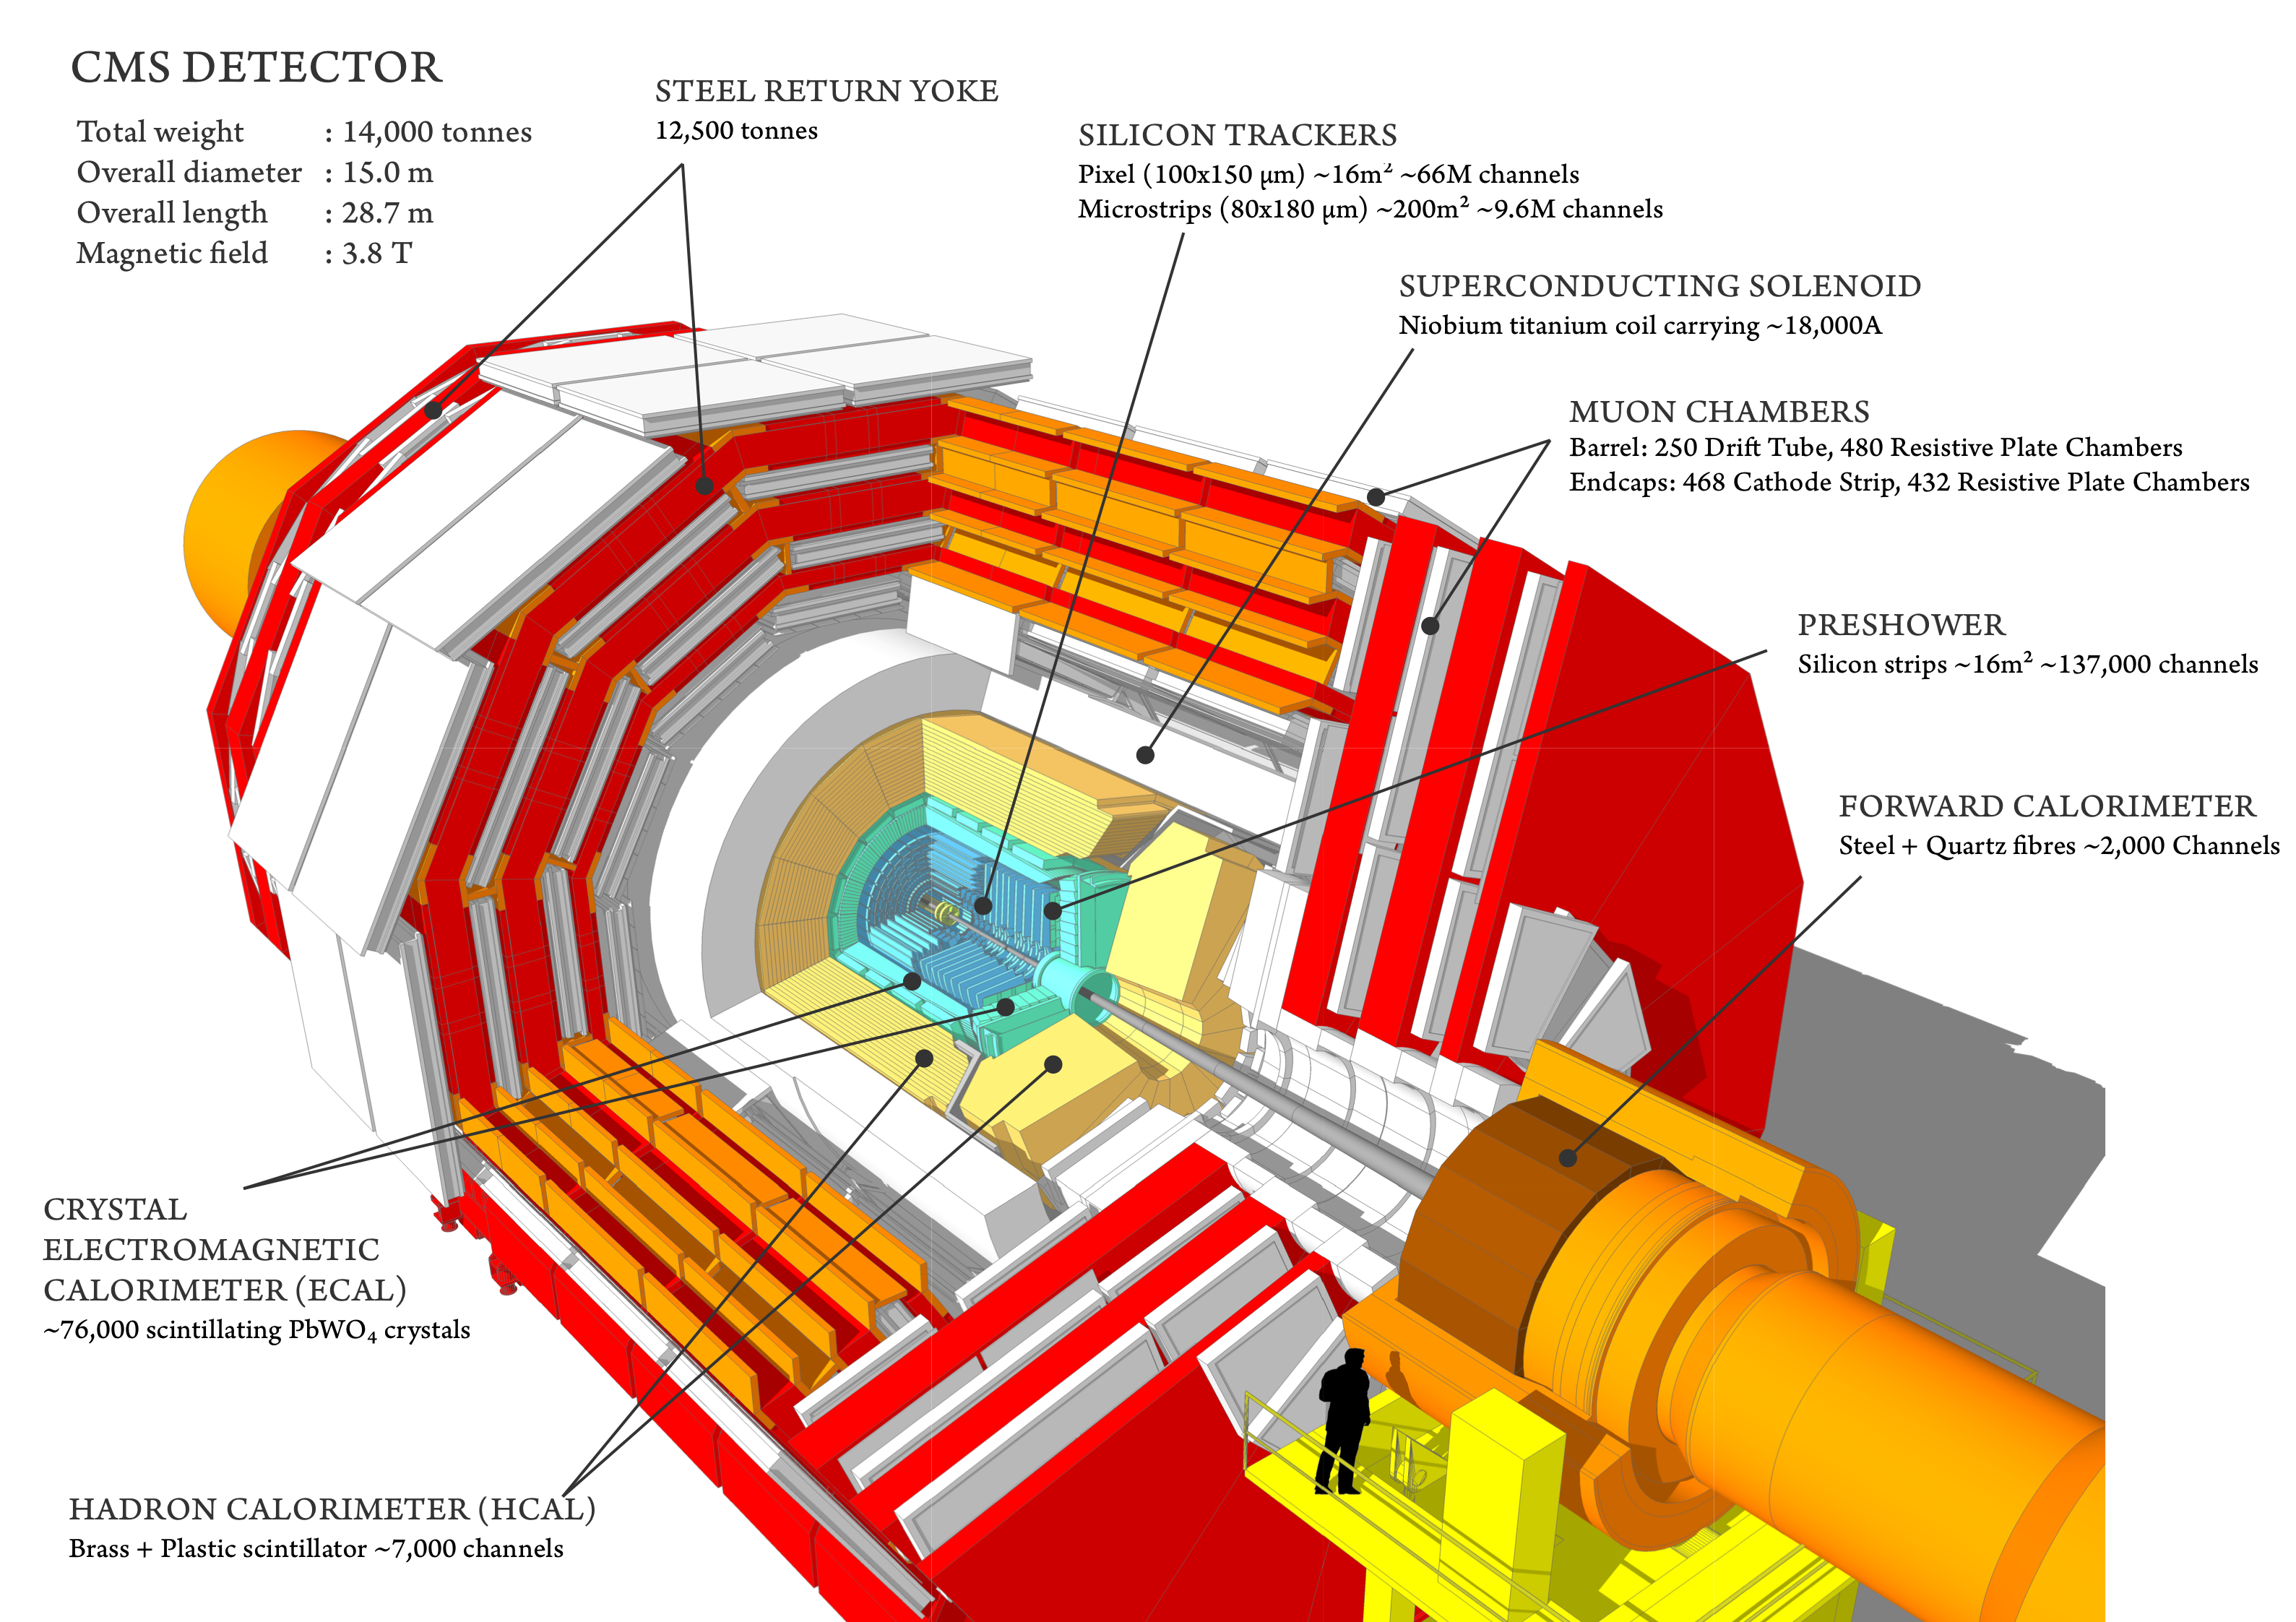
\includegraphics[width=\textwidth]{experiment/cmsWhole.png}
  \caption{
    Cutout schematic of CMS with all major subdetectors, the beamline, the magnet, and the return yoke visible. Reproduced from Ref.~\cite{Sakuma:1626816}.
  }\label{fig:cmsWhole}
\end{figure}

\subsection{Terminology and Geometry}
The CMS detector systems are arranged in cylindrical layers with the interaction point at the center, serving as the origin for the coordinate system.
The coordinate system is defined with the positive-$x$ direction pointing toward the center of the ring, positive-$y$ pointing vertically up, and positive-$z$ pointing parallel to the beam in the counterclockise direction when the LHC ring is viewed from above.
Particle momenta are typically expressed in quasicylindrical coordinates $\left(\pt,\eta,\phi\right)$.
Here $\pt$ is the magnitude of the particle's momentum transverse to the beam
\begin{equation}
  \pt \equiv \sqrt{p_x^2 + p_y^2},
\end{equation}
and $\phi$ is the azimuthal angle, i.e.\ the angle from the $x$-axis to the particle's trajectory in the $x$-$y$ plane.
The pseudorapidity~$\eta$ is defined as
\begin{equation}
  \eta \equiv -\ln \left[\tan\left(\frac{\theta}{2}\right)\right]
\end{equation}
where $\theta$ is the polar angle measured from the $z$-axis.
The relativistic rapidity
\begin{equation}
  y \equiv \frac{1}{2} \ln \left(\frac{E+p_z}{E-p_z}\right),
\end{equation}
converges to the pseudorapidity in the limit of massless particles.
Pseudorapidity is preferred to rapidity because it is purely geometrical, with no dependence on the particle energy.
Both are preferred over $\theta$ because rapidity differences are invariant under longitudinal boosts, and because hadron flux at colliders is roughly constant as a function of rapidity.
The transverse energy~$\et$ is the the magnitude of the particle's four-momentum transverse to the beam, equal to $\pt$ in the limit of massless particles.
Spatial coordinates are expressed as $\left(r,\eta,\phi\right)$, where $r$ is the distance from the beam in the $x$-$y$ plane.


\subsection{Magnet and Inner Tracking System}
A particle of charge $q$ moving through a uniform magnetic field of strength $B$ that points in the $z$ direction will travel in a helix of radius $R$, given by
\begin{equation}
  R = \frac{\pt}{\lvert q\rvert B},
\end{equation}
with the chirality of the helix determined by the sign of $q$.
Thus one can determine the transverse momentum of the particle by measuring its path through the magnetic field and finding the radius of curvature.
In practice, all but the lowest-energy particles leave too short an arc in the detector for direct measurement of the radius, so the sagitta of the arc is used instead, given by
\begin{equation}
  s = \frac{qBL^2}{8\pt}
\end{equation}
where $L$ is the length of the chord spanning the arc (typically equal to the radius of the tracking system).
The transverse momentum resolution varies as
\begin{equation}
  \frac{\delta \pt}{\pt} \propto \frac{\pt}{BL^2},
\end{equation}
so a strong field and a large tracking volume are vital to keeping measurements precise even at high energies.

To this end, CMS contains the world's largest superconducting magnet\footnote{Largest in the sense of having the largest stored energy when at constant full field. The largest by size is the ATLAS barrel toroid.}, a solenoid $13\unit{m}$ long and $6\unit{m}$ in diameter, which generates a nearly-uniform $3.8\unit{T}$ field in the centralmost part of the detector.
To measure the paths of charged particles in the field, the volume closest to the interaction point contains layers of silicon sensors that detect hits from charged particles with high efficiency and excellent position resolution, between $4.4\unit{cm}$ and $1.1\unit{m}$ from the beam for $2.7\unit{m}$ on either side of the interaction point.
This system, called the inner tracker and shown schematically in Fig.~\ref{fig:tracker}, consists of an inner pixel detector surrounded by a larger silicon strip detector.
Both consist of concentric cylinders of sensors covering the barrel of the detector capped by discs covering the high-$\eta$ region, up to $\abseta < 2.5$.
With a total of roughly $200\unit{m}^2$ of silicon, the inner tracker is the largest silicon tracker in the world.
Tracks may be reconstructed with hits in as many as 14 layers.
The downside of this is that the tracker represents a substantial amount of material for electrons and photons to interact with before they reach the calorimeters, with total material budget between 0.4 radiation lengths ($\eta=0$) and 1.8 radiation lengths ($\abseta \approx 1.4$), as shown.
The tracker-only $\pt$ uncertainty is around~1.2\% at $200\GeV$ and 15\% at~$1\TeV$.
Tracker readout is too slow for it to be used in the L1 trigger (see Section~\ref{sec:l1trig}), so the other systems must be used for this purpose.

\begin{figure}[h]
  \centering
  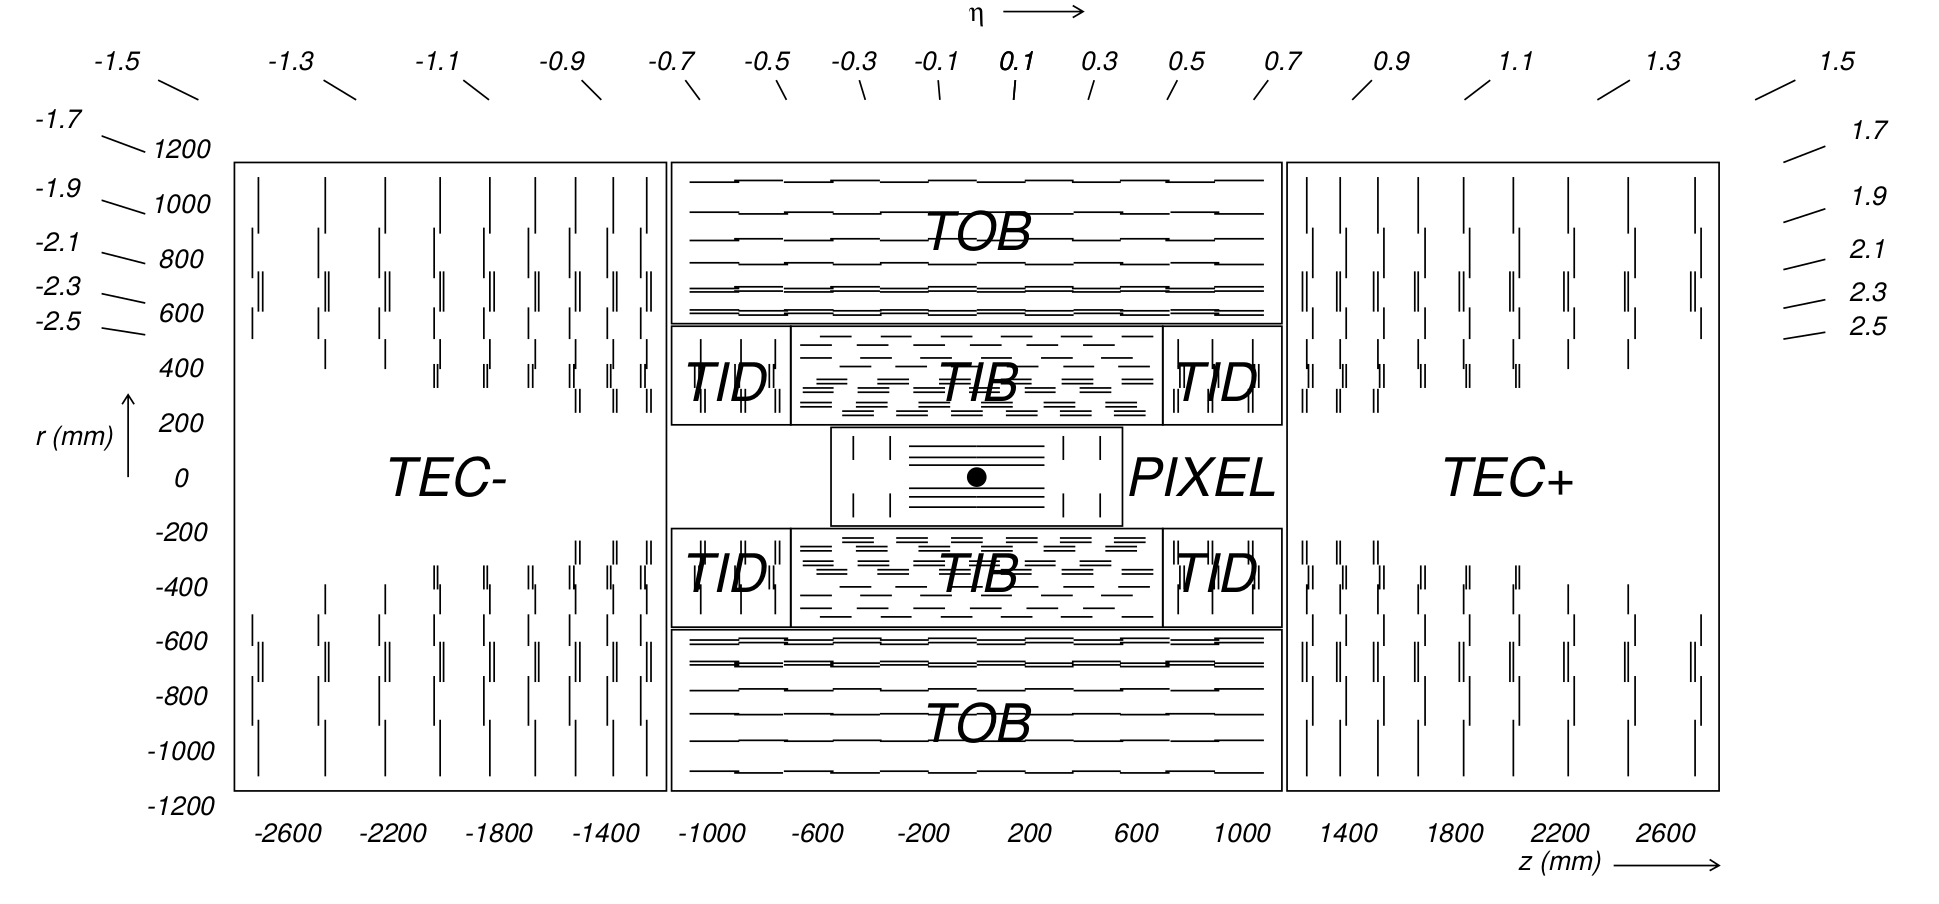
\includegraphics[width=\textwidth]{experiment/tracker.png}
  \caption{
    Diagram of the inner tracker layout, reproduced from Ref.~\cite{Chatrchyan:2008zzk}.
  }\label{fig:tracker}
\end{figure}


\begin{figure}[h]
  \centering
  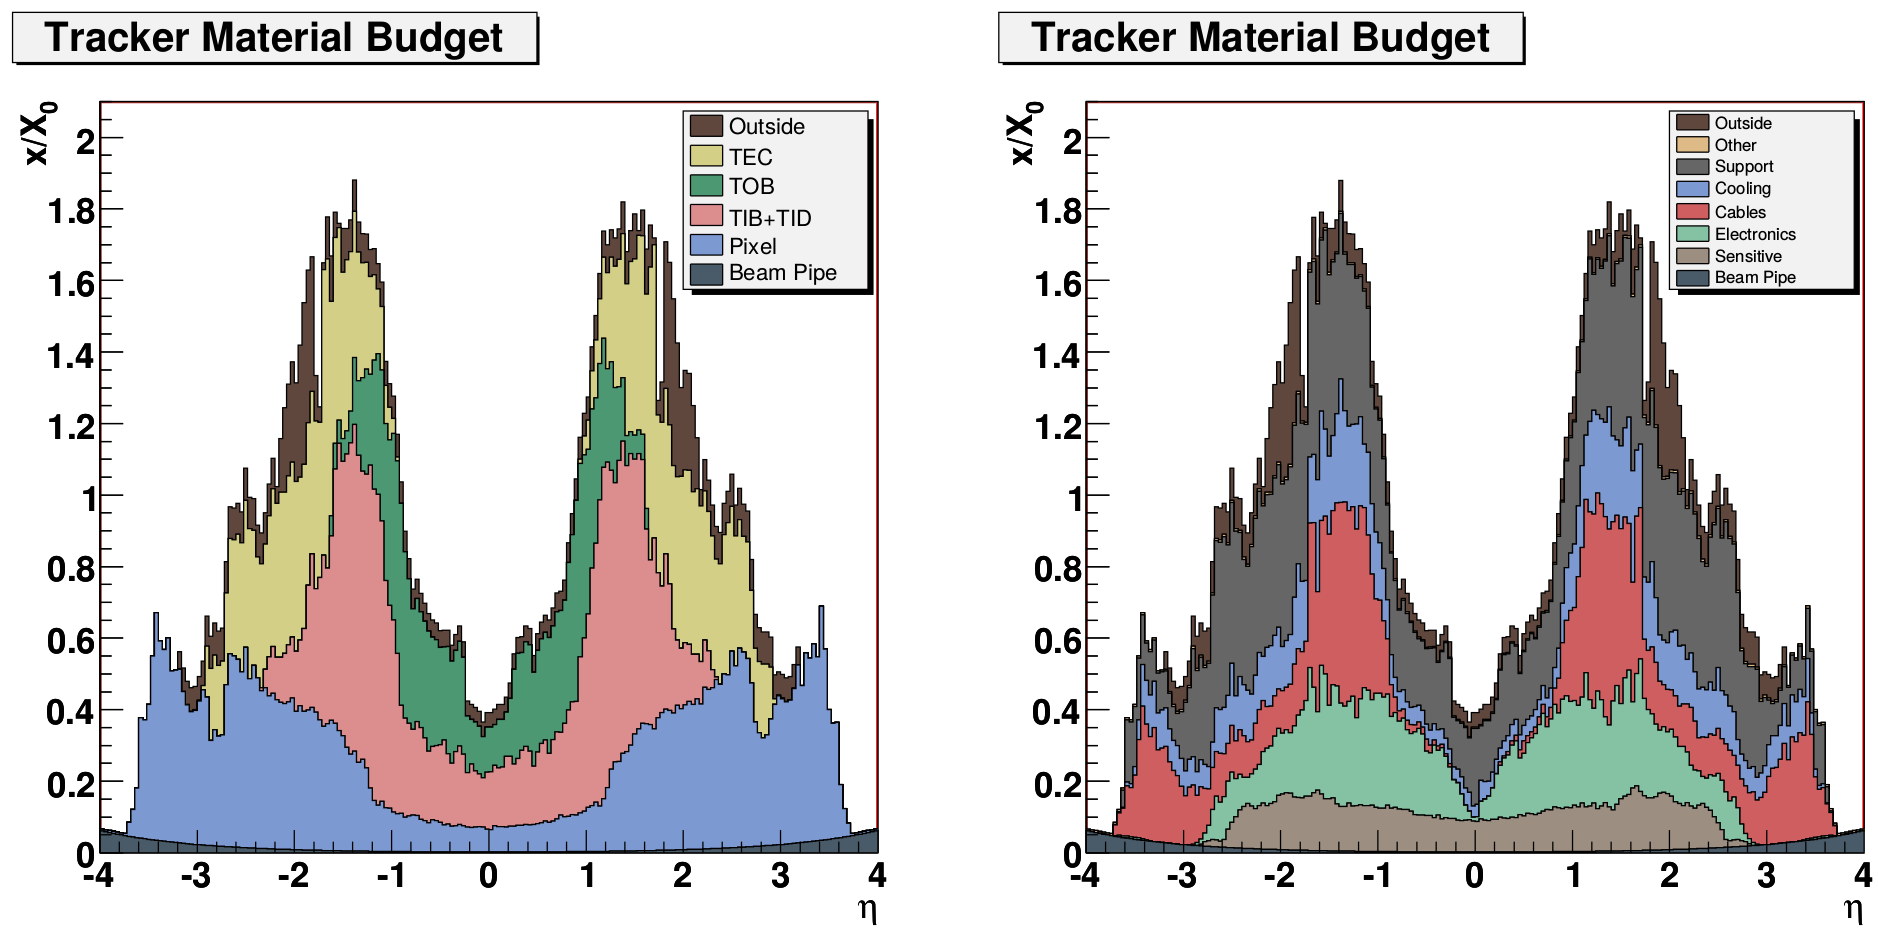
\includegraphics[width=\textwidth]{experiment/trackerMaterial.png}
  \caption{
    Total tracker material budget in units of electromagnetic radiation lengths, as a function of pseudorapidity.
    At (left) the total is divided by detector subsystem, at (right) by the function of the material. Reproduced from Ref.~\cite{Chatrchyan:2008zzk}.
  }\label{fig:trackerMaterial}
\end{figure}


\subsubsection{Pixel Detector}
The pixel detector, consisting of three layers in the barrel and two in the endcap, is responsible for accurate reconstruction of primary proton-proton interaction vertices and secondary vertices from $\Pqb$-meson decays, as well as providing ``seed'' tracks that may be used in strip tracker reconstruction.
As the system closest to the interaction point, the pixel system experiences the highest charged-particle flux must have extremely fine granularity to differentiate between nearby particles.
The 66~million pixels in the system have a cell size of $100 \times 150\unit{\mu m}^2$.
Interpolation of the analog signals from the individual pixels allows a final spatial resolution of $15\unit{\mu m}$ in each direction.
The outermost barrel layer is $10.2\unit{cm}$ from the beam, and the second endcap disk is $46.5\unit{cm}$ from the interaction point.
The sensor modules are arranged such that at least three sensors cover the solid angle within the pixels' acceptance.


\subsubsection{Strip Tracker}
Outside the pixels is the silicon strip tracker, extending out to $1.1\unit{m}$ in the $r$ direction and $\pm 2.8\unit{m}$ in the $z$ direction.
The tracker is divided into inner and outer subdetectors, each of which has both barrel cylinders and endcap discs.
In total, there are ten layers in the barrel and nine in each of the endcaps.
The inner tracker uses $320\unit{\mu m}$-thick sensors with a typical strip cell size of $10\unit{cm} \times 80\unit{\mu m}$, leading to hit resolutions of 23--$35\unit{\mu m}$.
The outer tracker uses $500\unit{\mu m}$-thick sensors with typical strip sizes up to $25\unit{cm} \times 180\unit{\mu m}$, leading to hit resolutions of 35--$53\unit{\mu m}$.


\subsection{Electromagnetic Calorimeter}
Outside of the tracker is the electromagnetic calorimeter (ECAL), which is designed to absorb and measure the energy of electrons and photons.
ECAL is made of 68,524 lead tungstate (\pbwo) crystals arranged in a cylindrical barrel (EB) covering $\abseta < 1.444$ and two endcap discs (EE) covering $1.566 < \abseta < 3.0$.
The geometry of the ECAL barrel and endcap can be seen in Fig.~\ref{fig:ecal}; the small gap between the barrel and endcap is necessary to accommodate cabling and support structures for the tracker.
\pbwo{} crystals scintillate blue-green light and are optically transparent, so the resulting light can be read out by avalanche photodiodes (APDs) in the barrel and vacuum phototriodes (VPTs) in the endcap.
ECAL's granularity is set by \pbwo's small {Moli\`ere} radius of~$2.2\unit{cm}$, which is also the size of the square front faces of the barrel crystals, which flare out to $2.6\unit{cm}$ at the back, giving them a truncated pyramid shape covering a roughy $0.0174 \times 0.174$ area of $\eta$-$\phi$ space.
The endcap crystals go from $2.86\unit{cm}$ squares at the front to $3.0\unit{cm}$ at the back.

\begin{figure}[h]
  \centering
  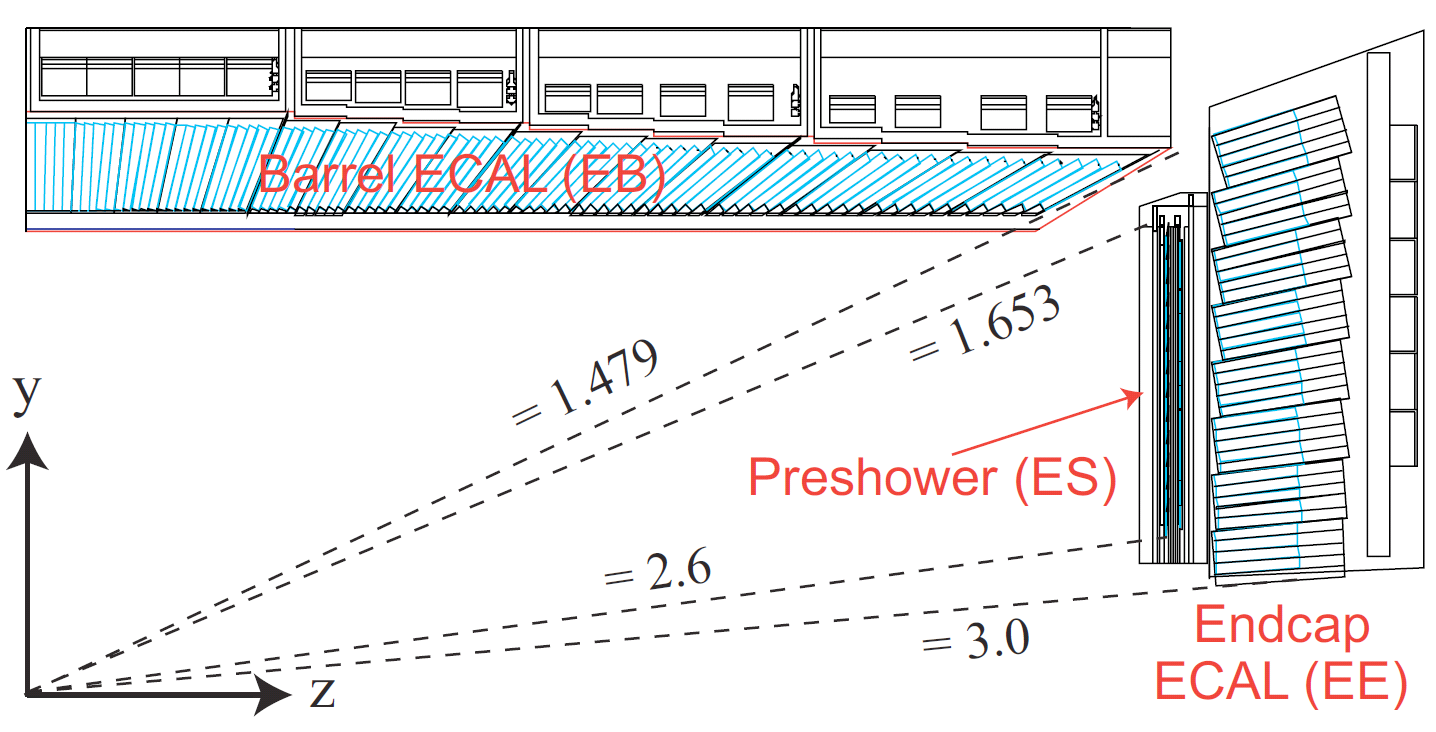
\includegraphics[width=0.7\textwidth]{experiment/ecal.png}
  \caption{
    Diagram of ECAL geometry, reproduced from Ref.~\cite{Isildak:2013kfa}.
  }\label{fig:ecal}
\end{figure}

One of the primary design innovations of CMS---the eponymous compactness---was to place the calorimetry inside the magnet so that tracks can be unambiguously associated with energy deposits in the calorimeters without interference from scattering in the magnet coils.
This is possible in part thanks to the high density ($8.28\unit{g}/\unit{cm}^3$) and short radiation length ($0.89\unit{cm}$) of \pbwo, which allow ECAL crystals to be only $23\unit{cm}$ long in the barrel and $22\unit{cm}$ long in the endcap while still spanning 25.8 and 24.7 radiation lengths, respectively.
This is enough to ensure that essentially no electrons or photons escape ECAL with any appreciable remaining energy.

The total scintillation light yield is relatively low, averaging just 4.5~photons per~$\MeVns$ deposited,
The Poisson fluctuations in the yield are the largest contribution to ECAL energy resolution for most electron and photon energies, represented by the first term in the full resolution equation,
\begin{equation}
  \left(\frac{\delta E}{E}\right)^2 = \left(\frac{2.8\%}{\sqrt{E/\GeVns}}\right)^2 + \left(\frac{0.12}{E/\GeVns}\right)^2 + \left(0.30\%\right)^2.
\end{equation}
The second term comes from electronic noise and noise from pileup, and the last term represents intrinsic differences between crystals.
The upside to \pbwo's scintillation is that it is fast: roughly 80\% of the light is emitted in the $25\unit{ns}$ between bunch crossings.


\subsection{Hadronic Calorimeter}
Between ECAL and the magnet is the hadronic calorimeter (HCAL), responsible for measuring the energy of hadronic jets.
HCAL is a sampling calorimeter, meaning that the hadrons pass through dense, uninstrumented material and the products of the resulting interactions deposit energy in scintillators which are used to measure the total energy of the original incoming particles.
The HCAL barrel (HB, $\abseta < 1.305$) and endcap (HE, $1.305 < \abseta < 3.0$) are made of layers of brass absorber interleaved with plastic scintillating tiles.
The energy resolution in HB and HE is given by
\begin{equation}
  \label{eq:HBHE_resolution}
  \left(\frac{\delta E}{E}\right)^2 = \left(\frac{90\%}{\sqrt{E/\GeVns}}\right)^2 + \left(4.5\%\right)^2.
\end{equation}
The first term is from the stochastic evolution of hadronic showers in the absorber, the second is from calibration uncertainties.

Because HB is not enough to absorb all hadrons in the barrel, there is an extra outer HCAL component (HO) outside of the magnet, consisting of two more layers of scintillator on either side of a $20\unit{cm}$-thick iron ``tail catcher'' covering $\abseta < 1.3$.
The geometry of HB, HE, and HO is shown in Fig.~\ref{fig:hcal}.
The thickness of HB and HE is constrained by the size of the magnet, varying from 5.4 nuclear interaction lengths in the central barrel to more than 10 in the endcaps.
With HO and the 1.1 interaction lengths in ECAL considered, no part of the calorimeter system spans fewer than 11.8 interaction lengths except in the gaps between barrel and endcap, minimizing the flux of hadronic ``punchthrough'' interacting with the muon system.
The total material budget in front of the layers of the muons systems is shown in Fig.~\ref{fig:hcalMaterial}.

\begin{figure}[h]
  \centering
  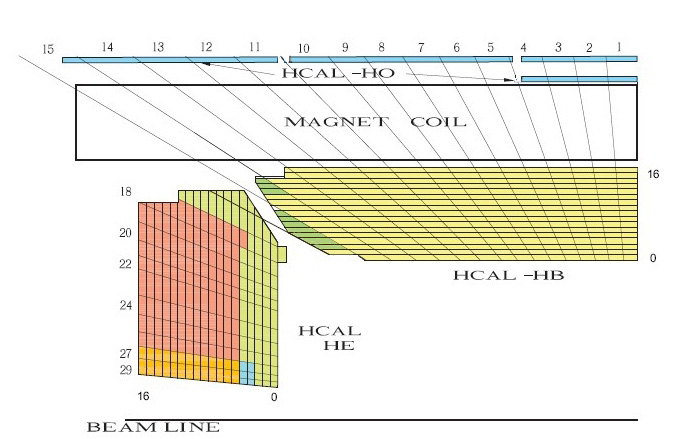
\includegraphics[width=\textwidth]{experiment/hcal.png}
  \caption{
    Diagram of HCAL geometry, reproduced from Ref.~\cite{Chatrchyan:2008zzk}.
  }\label{fig:hcal}
\end{figure}

\begin{figure}[h]
  \centering
  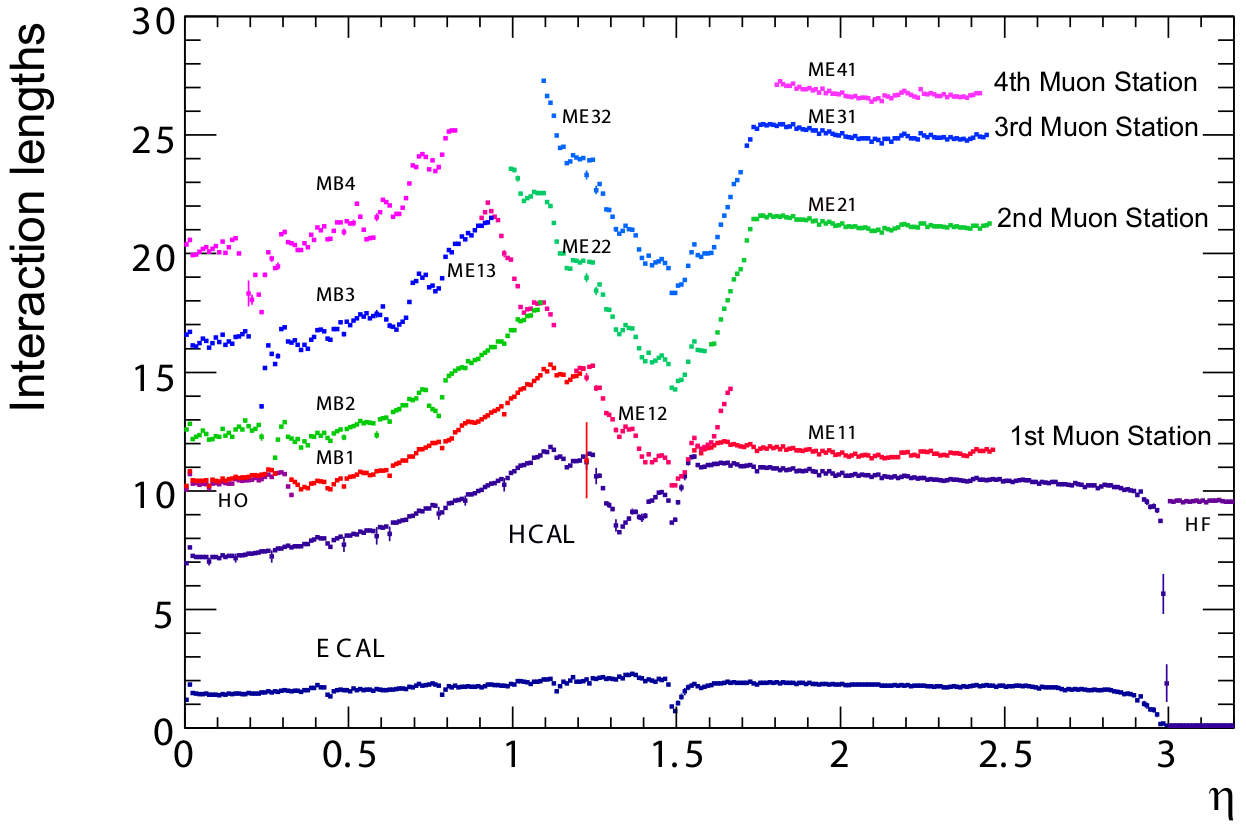
\includegraphics[width=0.7\textwidth]{experiment/hcalMaterial.png}
  \caption{
    Total material budget in units of nuclear interaction lengths, as a function of pseudorapidity, reproduced from Ref.~\cite{Chatrchyan:2008zzk}.
  }\label{fig:hcalMaterial}
\end{figure}

Closer to the beam line on each side, the forward hadronic calorimeter (HF, $3.0 < \abseta < 5.2$) is made of iron instead of brass to maximize radiation hardness and acts as a Cherenkov detector with quatz fibers as the active detection element.
Half the fibers extend the entire depth of HF, while the other half start after the hadrons have traversed $22\unit{cm}$ of iron, allowing electromagnetic and hadronic energy to be differentiated without ECAL\@.
The energy resolution in HF is given by
\begin{equation}
  \left(\frac{\delta E}{E}\right)^2 = \left(\frac{172\%}{\sqrt{E/\GeVns}}\right)^2 + \left(9\%\right)^2,
\end{equation}
where the terms have the same physical interpretation as those in Eq.~\ref{eq:HBHE_resolution}.
HF improves CMS's missing energy resolution by roughly a factor of three.


\subsection{Muon Spectrometer}
Many of the most interesting physics processes at the LHC involve high energy muons, so muon identification, triggering, and momentum measurement are important design goals.
Muons leave very little energy in the calorimeters, so ECAL and HCAL cannot be used for triggering and identification as they are for electrons, photons and hadrons, or to improve momentum measurements of high-$\pt$ muons whose tracks are too straight to allow good measurements of their curvature.
Instead, these functions are provided for muons by three gas-based systems surrounding the rest of the detector.
In all three, ionizing gas chambers provide hits which form a track.
The magnetic field for this is provided by the return yoke, a set of steel plates interleaved with the muon chambers which confine the solenoid's magnetic field.
The yoke plates weigh a total of $10,000\unit{t}$ and are fully saturated by the solenoid.

Unlike the inner tracker, the muon systems can be read out fast enough to provide triggering.
Because muons above $3\GeV$ generally traverse the muon system while most other measurable particles are stopped in the calorimeters, magnets, or return yoke, the muon system provides high efficiency, low-background muon identification.
The muon system's momentum measurements are not competitive with the inner tracker's at low $\pt$, but a combined fit of the inner track and the muon system (``standalone'') track improves muon $\pt$ resolution above roughtly $200\GeV$.
The geometry of all three muon systems and the return yoke can be seen in Fig.~\ref{fig:muonSystem}.

\begin{figure}[h]
  \centering
  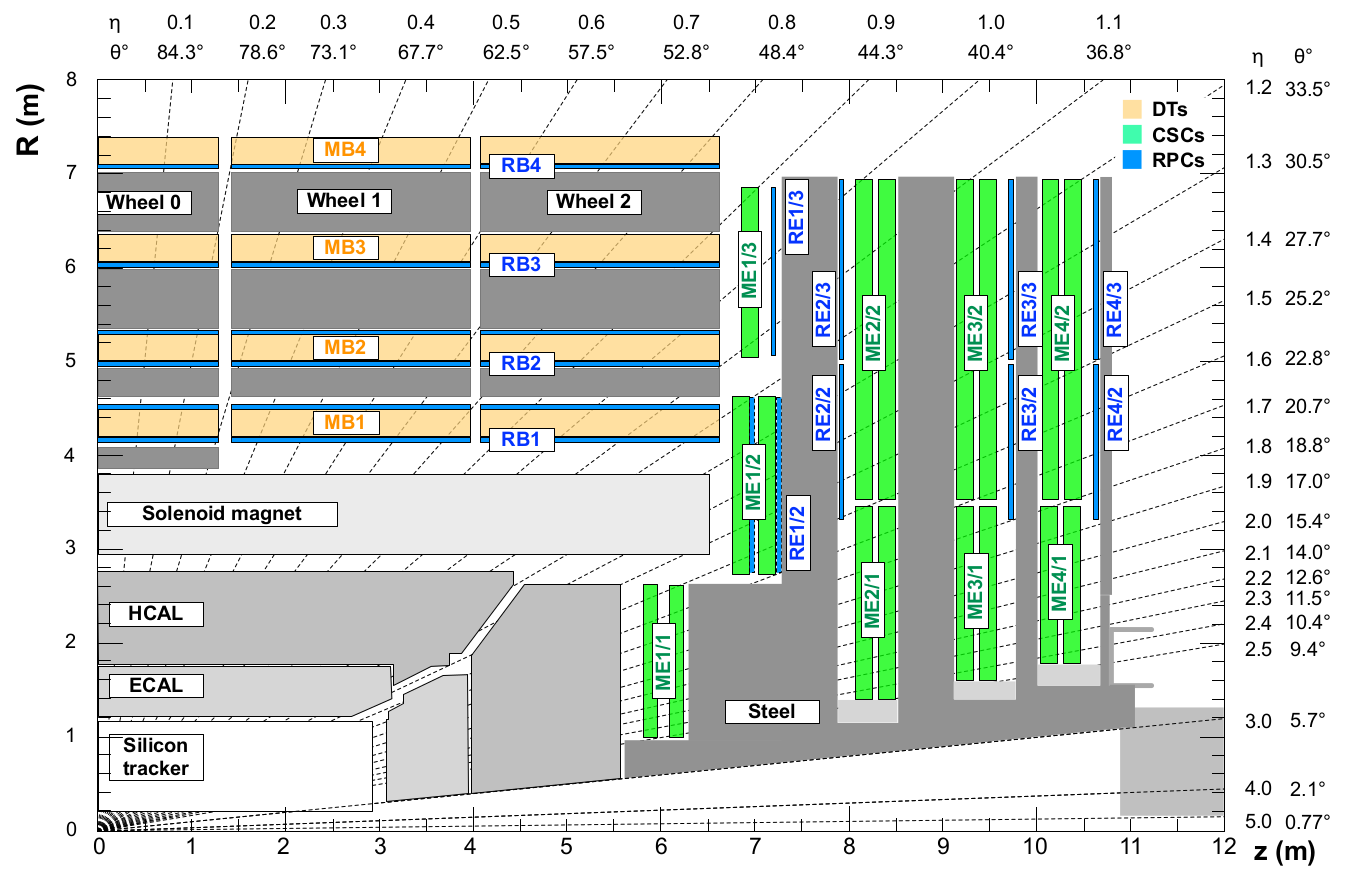
\includegraphics[width=\textwidth]{experiment/muonSystem.png}
  \caption{
    Diagram of muon system and return yoke geometry, reproduced from Ref.~\cite{Abbiendi:2015txa}. The magnet, calorimeters, and inner tracker are also visible.
  }\label{fig:muonSystem}
\end{figure}


\subsubsection{Drift Tubes}
In the barrel ($\abseta < 1.2$), drift tube (DT) chambers are arranged in four ``stations'' separated by layers of the yoke.
Stations are made of two or three superlayers (SLs) of four layers of rectangular drift cells.
Adjacent layers are staggered latterally by half a cell width to avoid gaps.
Each station has two SLs with wires running parallel to the beam to measure muon tracks in the $r$-$\phi$ plane, separated by an aluminum honeycomb lattice to provide mechanical rigidity and act as a spacer.
The inner three stations contain an extra SL on the outer side of the spacer with wires perpendicular to the beam line, to measure muon position along the $z$-axis.

Each drift cell contains a roughly $2.4\unit{m}$-long wire in gas (85\% Ar, 15\% CO$_2$).
The electric field in the cell is proveded by aluminum tape glued to the top and bottom of the cell and held at $+1.8\unit{kV}$ relative to the grounded aluminum plates above and below.
Aluminum tape cathodes on the side of the cell are held at $-1.2\unit{kV}$, while the wires act as $+3.6\unit{kV}$ anodes.
The width of each cell perpendicular to muon motion, $42\unit{mm}$, was chosen for a maximum drift time of $380\unit{ns}$, sufficient to obviate the need for double-hit readout logic in this low-occupancy region of the detector.
The height of $13\unit{mm}$ set by mechanical and space constraints.
Track timing resolution in each SL is a few nanoseconds when all cells are allowed to read out all deposited charge.
The $r$-$\phi$ position resolution available for online use in the trigger is about $1.5\unit{mm}$ in each SL\@; offline, for a single wire it is roughly $250\unit{\mu m}$, leading to an overall resolution of $100\unit{\mu m}$ at each station.


\subsubsection{Cathode Strip Chambers}
Muons with $1.2 < \abseta < 2.4$ are detected by the cathode strip chambers (CSCs).\footnote{Where the CSCs and DTs overlap ($0.9 < \abseta < 1.2$), tracks are formed from hits in both.}
The CSC system's trapezoidal chambers are arranged on discs interleaved with the endcap yoke in four layers.
Chambers close to the beamline each cover $20\degree$ sections in $\phi$, outer chambers cover $10\degree$ sections, with overlap to avoid gaps.

A CSC chamber is made of seven panels sandwiched together to make six gaps filled with a gas mixture (40\% Ar, 50\% CO$_2$, 10\% CF$_4$).
Six of the plates have cathode strips milled into one side, varying in pitch from $8.4\unit{mm}$ at the narrow end of the trapezoid to $16\unit{mm}$ at the wide end, with $0.5\unit{mm}$ gaps between strips.
Three panels are wrapped with anode wires, alternating with the other panels so that every gas gap has a plane of wires.
Wires are spaced $3.2\unit{mm}$ apart and run azimuthally around the detector, except for the innerpost chamber closest to the interaction point, which are inside the magnet and must have their wires tilted $29\degree$ so that charge collected by the wires moves parallel to them despite the Lorentz forces from the solenoid.

A typical muon will deposit charge in 3--4 cathode strips and a similar number of anode wires per gas gap, allowing hit position to be interpolated using all these signals as well as timing information.
The single-plane spatial resolution can be as good as $80\unit{\mu m}$ but depends strongly on where in the width of the strip the muon hits.
The strips in alternating planes are therefore offset by half their width.
Measurements from all six gas gaps in a chamber are combined into a segment with position resolution in the 30--$80\unit{\mu m}$ range, which depends on the chamber but not where in the chamber the muon hit.

Anodes and cathodes are held $3.6\unit{kV}$ from each other, leading to a drift time of roughly $300\unit{ns}$.
Single anode planes have an RMS timing resolution of around $11\unit{ns}$, insufficient for assigning a hit unambiguously to an individual bunch crossing, as required for triggering.
However, information from all six anode planes in a chamber can be combined to yield a segment timing resolution around $5\unit{ns}$.
Segments are therefore the unit of information sent to the trigger.
Segment position resolution at trigger level is 1--$2\unit{mm}$.


\subsubsection{Resistive Plate Chambers}
To provide a redundant set of muon momentum measurements, as well as precise timing of muon hits, CMS has six layers of resistive plate chambers (RPCs) in the barrel and four in the endcap up to $\abseta < 1.6$.
RPC chambers consist of two thin layers of intert gas (95.2\% C$_2$H$_2$F$_4$, 4.5\% C$_4$H$_{10}$, 0.3\% SF$_6$) each between a pair of Bakelite electrodes held at $9.3\unit{kV}$.
The two ``gas gaps'' are placed on either side of a plane of copper strips.
When a passing muon ionizes the gas, the high voltage causes a fast electron avalanche read out by the strips.
The narrow gap allows the RPCs to have single-hit timing resolution around $1\unit{ns}$, but the spatial resolution is limited to about $1\unit{cm}$ by the size of the readout strips.
The DTs and CSCs both have better momentum resolution than the RPCs, but RPCs are a simple, robust auxiliary system and the timing resolution can be used in conjunction with the other systems to improve overall muon measurements.


\subsection{Data Acquisition and Trigger}
With a bunch crossing rate of $40\unit{MHz}$ giving a collision rate that can exceed $1.6\unit{GHz}$ and raw event sizes of 1--$2\unit{MB}$, the raw data generation rate of CMS could potentially be several PB/s, substantially more than can be read out, stored or analyzed with current technology.
However, most events consist only of low-energy, well-understood QCD interactions, so the data rate can be drastically reduced by reading out and storing only events likely to have interesting physics content.
CMS reduces the event rate with a two-level trigger system.

The level-1 (L1) trigger uses custom hardware operating on trigger primitives (TPs), low-granularity detector information, to reduce the event rate to $100\unit{kHz}$ or less.
Inner tracker readout is too slow for use in the trigger, so only the calorimeters and muon systems generate TPs.
Events accepted at level-1 are read out, digitized, and sent to the high level trigger (HLT), where they are partially reconstructed in software and filtered further, reducing the final rate of stored events to roughly $1\unit{kHz}$.


\subsubsection{Level-1 Trigger}\label{sec:l1trig}
LHC beams collide at too high a rate for trigger decisions to be made in software, so the L1 trigger is instead implemented in custon hardware, with processing done using field-programmable gate arrays (FPGAs) as much as possible for flexibility, and application-specific integrated circuits (ASICs) where required.
Hardware limitations of other CMS subsystems---in particular, the inner tracker's readout speed and buffer capacity---impose strict constraints on the system.
The rate of events passing at level-1 cannot exceed $100\unit{kHz}$ and the system's overall latency cannot exceed roughly $4.2\unit{\mu s}$.
These goals are achieved while maintaining high efficiency for interesting physics events by using only low-granularity detector information, to reduce the bandwidth needed within the trigger system.
Information flows through subsystems, with the amount of data reduced at each step.
Calorimeter and muon information are processed in parallel and combined only in the final step.
Optical links between systems provide high-bandwidth data transfer and allow flexibility in the overall trigger architecture.
The calorimeter trigger was upgraded with respect to the Run~I configuration in 2015, and the whole trigger system was overhauled in 2016~\cite{Tapper:1556311}.
Both configurations will be described here.

Calorimeter information is compressed into trigger primitives (TPs) for use in the trigger by trigger primitive generators (TPGs).
Each TP represents a ``tower'' consisting of a $5 \times 5$ cluster of barrel or endcap ECAL crystals and the portion of HCAL behind them, or a section of the HF\@.
The TP contains an 8-bit transverse energy sum and a quality bit for each calorimeter, and six bits of error checking and bookkeeping information.
In 2015, TPs were sent to the Regional Calorimeter Trigger (RCT), which processed 18 portions of the detector (segmeted in $\phi$ with $+\eta$ and $-\eta$ treated separately) in parallel in separate crates of electronics, using several ASICs and one FPGA in each crate for processing.
Each RCT crate summed the TPs with $\abseta < 3.0$ into $4 \times 4$ tower regions, and found isolated and non-isolated $2 \times 1$ tower $\Pe/\Pa$ and $\Pt$ candidates.
These objects were sent to Stage~1 Layer~2, which selected the best $\Pe/\Pa$ and $\Pt$ candidates from the entire detector, clustered regions into $3 \times 3$ region jet candidates, and computed global quantities like missing transverse energy and the scalar sum of transverse momentum for all particles in the event.
Pileup subtraction was performed with a lookup table (LUT) based on the number of regions in the detector with no energy.

In 2016, the whole calorimeter trigger was replaced with a new two-tiered system.
Stage~2 Layer~1 (``CaloL1'') consists of 18 FPGA-based Calorimeter Trigger Processor~7 (CTP7) cards, which calibrate and reformat the TPs before forwarding them to Stage~2 Layer~2 (``CaloL2''), an FPGA-based time-multiplexed system which finds $\Pe/\Pa$, $\Pt$, and jet candidates and computes global quantities for whole events in parallel using tower-level information.

In 2015, the DTs and CSCs fed track segments into track finders (DTTF and CSCTF) which used pattern recognition algorithms to reconstruct tracks and measure their $\pt$, sharing information between the track finders to avoid inefficiency in the overlap region.
The RPCs made their own tracks.
Since the 2016 upgrade, track finding has been done by geometrical region of the detector rather than detector subsystem alone, with separate track finders for the barrel (BMTF, $\abseta < 0.85$), endcap (EMTF, $1.25 < \abseta < 2.4$) and overlap (OMTF, $0.85 < \abseta < 1.25$) regions.
The track finders feed into the Global Muon Trigger (GMT, upgraded to $\mu$GMT in 2016), which merges and sorts tracks, analyzes their quality and selects the best ones.

The calorimeter and muon trigger systems, which have up to this point worked entirely in parallel, both send their selected candidates and global quantities to the Global Trigger (GT, upgrated to $\mu$GT).
The Global Trigger contains the trigger menu, the configurable set of algorithms used to determine whether an event is accepted or not.
These algorithms can use combinations of the objects from the calorimeter and muon trigger systems, including imposing topological requirements, e.g.\ requiring a large $\Delta\eta$ between muons in a pair.
The final decision is a logical OR of all triggers in the menu, but each trigger may be prescaled, i.e.\ only included in the final decision a fraction of the time in order to reduce its rate.
When an event is accepted, a level~1 accept (L1A) signal is sent to all CMS subsystems instructing them to read out information collected in the accepted event, which is stored in buffers until it can be read out or safely discarded.
A diagram of the whole 2016 L1 trigger system and its information flow is shown in Fig.~\ref{fig:triggerFlow}.

\begin{figure}[h]
  \centering
  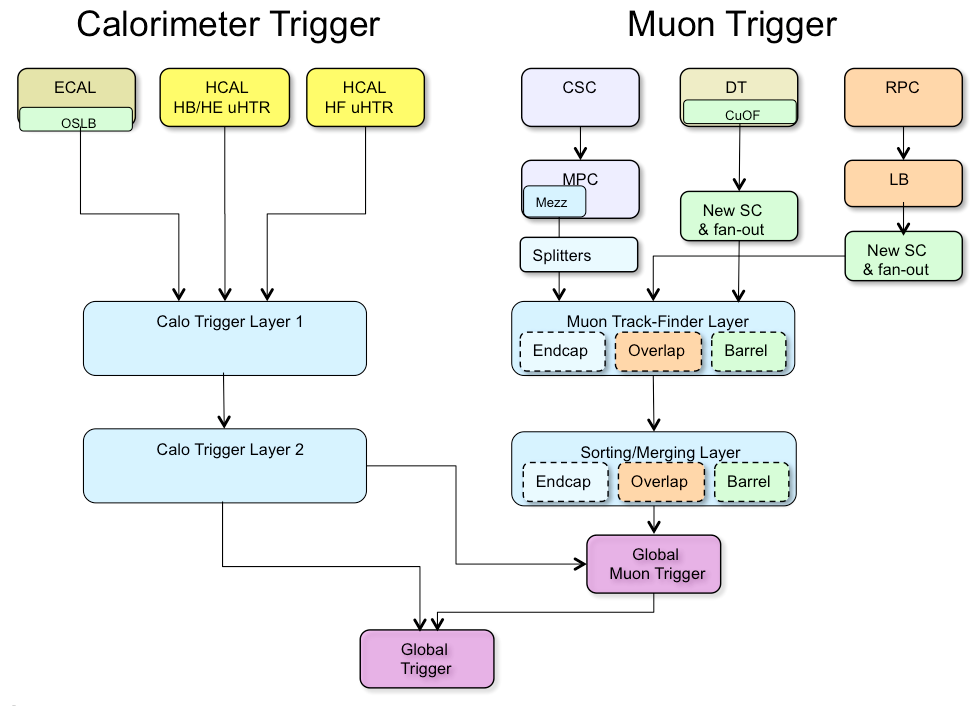
\includegraphics[width=\textwidth]{experiment/triggerFlow.png}
  \caption{
    Data flow diagram for the CMS L1 trigger after the 2016 overhaul, reproduced from Ref.~\cite{Tapper:1556311}.
  }\label{fig:triggerFlow}
\end{figure}


\subsubsection{High-Level Trigger}
After an accepted event is read out and digitized, it must undergo another level of screening before being stored.
The High Level Trigger (HLT) uses full detector information reconstructed with versions of the normal CMS reconstruction algorithms specially optimized for speed, running on a large farm of commercial computers.
Much of HLT's power comes from having tracker information, allowing more precise momentum measurements, isolation calculations and identification algorithms than are available at L1.
For example, the pixels can be used to reconstruct vertices and tag $\Pqb$-quark jets, and requirements can be placed on the invariant mass of a lepton pair.
However, track reconstructions is slow, so it is typically only done as one of the last steps in the filtering process, allowing the event to be rejected based on more easily reconstructed objects like tracks in the muon system.
Other optimizations include only reconstructing tracks near objects passed in by the L1 Global Trigger.
The final result is that the rate of events saved for later analysis is around $1\unit{kHz}$.


\subsection{Luminosity Determination}
A precise measurement of the luminosity delivered by the LHC is critical to precisely measuring any cross section.
The instantaneous luminosity for $n_b$ colliding bunch pairs with intensity $N_b$ and orbit frequency $f_\textit{rev}$ is given by
\begin{equation}\label{eq:lumiByAeff}
  \lumiL = \frac{n_b N_b^2 f_\textit{rev}}{A_\text{eff}}
\end{equation}
where $A_\text{eff}$ is the effective area of the beam-beam overlap.
If beam $i$ has a gaussian density profile in the $u$ direction of width $\sigma_{i,u}$, and the beam densities are uncorrelated in each direction, then
\begin{equation}
  A_\text{eff} = 2\pi \sqrt{\sigma_{1,x}^2 + \sigma_{2,x}^2} \sqrt{\sigma_{1,y}^2 + \sigma_{2,y}^2}.
\end{equation}
The beam widths $\sigma_{i,u}$, the only unknowns in Eq.~\ref{eq:lumiByAeff}, are purely geometrical and can be found with the Van de Meer (VdM) scan method~\cite{vanderMeer:1968zz,Zanetti:1357856}.
In a VdM scan, for which LHC has a special run mode, one beam is held fixed while the position of the other is scanned in the $x$-$y$ plane, and detector activity is measured as a function of beam displacement.
Because the width of the interaction rate distribution is independent of its overall normalization, the detector activity metric may be any quantity linearly proportional to the interaction rate.

Over the course of an LHC run, $n_b$, $N_b$, and $A_\text{eff}$ are all subject to change, and in fact the VdM scans are performed with a special LHC configuration, so in practice the procedure outlined above provides a calibration and overall scale for luminosity measurements during physics collisions.
For a given detector metric labeled $Q$ with rate $R^Q$ that peaked at $R_0^Q$ with no beam displacement, the VdM scan yields a visible cross section, the constant of proportionality between the rate and the instantaneous luminosity,
\begin{equation}
  \sigma_\text{vis}^Q \equiv \frac{R^Q}{\lumiL} = A_\text{eff} R_0^Q.
\end{equation}
CMS has several such metrics; the primary one used for measuring integrated luminosity is the number of pixel hit clusters~\cite{CMS-PAS-LUM-15-001,CMS-PAS-LUM-17-001}.
The instantaneous luminosity is given by
\begin{equation}
  \lumiL = \frac{\langle N_c \rangle f_\textit{rev}}{\sigma_\text{vis}^\text{PCC}} = \frac{\langle N_c \rangle}{A_\text{eff} \langle N_c \rangle_0}
\end{equation}
where $\langle N_c \rangle$ is the average number of pixel hit clusters at each bunch crossing and $\langle N_c \rangle_0$ is its peak value during the VdM scan.

A number of complications must be accounted for or included in systematic uncertainty estimates.
Beam-beam interation effects, correlations between the proton density distributions in the $x$ and $y$ directions, drifts in the beam orbit, and normalization uncertainties on the bunch intensity and absolute distance scale from the beam spot must all be handled with care.
The result is a total integrated luminosity uncertainty of $2.3\%$ in 2015 and $2.5\%$ in 2016\@.
